\documentclass[12pt,a4paper]{article}

% ============ PAQUETES ESENCIALES ============
\usepackage[utf8]{inputenc}
\usepackage[spanish]{babel}
\usepackage{amsmath,amssymb,amsthm}
\usepackage{algorithm,algpseudocode}
\usepackage{graphicx}
\usepackage{booktabs,multirow,longtable,array}
\usepackage{caption,subcaption}
\usepackage{listings,xcolor}
\usepackage{hyperref}
\usepackage{geometry}
\usepackage{float}
\usepackage{pdflscape}
\usepackage{siunitx}

\geometry{margin=2.5cm}

% ============ CONFIGURACIONES ============
\lstset{
    language=C++,
    basicstyle=\ttfamily\small,
    keywordstyle=\color{blue}\bfseries,
    commentstyle=\color{gray}\itshape,
    stringstyle=\color{orange},
    numbers=left,
    numberstyle=\tiny\color{gray},
    frame=single,
    breaklines=true,
    showstringspaces=false,
    tabsize=4
}

\hypersetup{
    colorlinks=true,
    linkcolor=blue,
    citecolor=blue,
    urlcolor=blue,
    pdftitle={Modelacion Epidemiologica SEIR con RK4},
    pdfauthor={Gregory Uzcategui}
}

% ============ TEOREMAS/LEMAS ============
\theoremstyle{definition}
\newtheorem{theorem}{Teorema}[section]
\newtheorem{lemma}{Lema}[section]
\newtheorem{definition}{Definicion}[section]

% ============ COMANDOS PERSONALIZADOS ============
\newcommand{\norm}[1]{\|#1\|}
\newcommand{\R}{\mathbb{R}}
\newcommand{\vect}[1]{\mathbf{#1}}
\newcommand{\dd}[2]{\frac{\mathrm{d}#1}{\mathrm{d}#2}}

% ============ DOCUMENTO ============
\begin{document}

% ---------- PORTADA ----------
\begin{titlepage}
    \centering
    \vspace*{2cm}
    {\Huge\bfseries Modelaci\'{o}n Epidemiol\'{o}gica y Sistemas Din\'{a}micos\\[0.3cm] Resoluci\'{o}n Num\'{e}rica del Modelo SEIR mediante RK4\par}
    \vspace{1.5cm}
    {\Large Informe T\'{e}cnico de Implementaci\'{o}n y Resultados\par}
    \vspace{2cm}
    {\Large Autor: Gregory Uzcategui / CI: 27.376.191 \par}
    \vspace{2cm}
    {\large
    \textbf{Stack tecnol\'{o}gico:} C++17 (Eigen 3.4), CMake, Python 3 (pandas, matplotlib)\\[0.5cm]
    \textbf{M\'{e}todo num\'{e}rico:} Runge-Kutta de 4to Orden (RK4) implementado desde cero\\[0.5cm]
    \textbf{Problema:} Simulaci\'{o}n del modelo SEIR con intervenci\'{o}n no farmac\'{e}utica y an\'{a}lisis de conservaci\'{o}n
    \par}
    \vfill
    {\large \today\par}
\end{titlepage}

% ---------- RESUMEN ----------
\begin{abstract}
\noindent
La implementaci\'{o}n de un solver num\'{e}rico para el modelo epidemiol\'{o}gico compartimental SEIR. Se desarroll\'{o} el algoritmo de Runge-Kutta de 4to orden (RK4) \textbf{desde cero} en C++17, utilizando la librer\'{i}a Eigen para la manipulaci\'{o}n eficiente de vectores de estado. Se evaluaron dos escenarios: uno libre ($\beta = 0.6$) y otro con intervenci\'{o}n de confinamiento ($\beta$ se reduce a $0.25$ en $t=30$). 
\end{abstract}

\tableofcontents
\newpage

% ---------- 1. INTRODUCCION ----------
\section{Introducci\'{o}n}\label{sec:intro}

La modelaci\'{o}n matem\'{a}tica de enfermedades infecciosas permite predecir el comportamiento de un brote y evaluar el impacto de intervenciones no farmac\'{e}uticas. El modelo SEIR es un sistema compartimental donde la poblaci\'{o}n total $N$ se divide en cuatro estados: Susceptibles ($S$), Expuestos ($E$), Infectados ($I$) y Recuperados ($R$). A diferencia del modelo SIR b\'{a}sico, el SEIR introduce un periodo de latencia donde el individuo est\'{a} infectado pero a\'{u}n no es contagioso.

\subsection{Justificaci\'{o}n de las Herramientas Tecnol\'{o}gicas}

\begin{itemize}
    \item \textbf{C++ y Eigen 3.4:} Se eligi\'{o} C++ por su alto rendimiento en c\'{a}lculo num\'{e}rico y control expl\'{i}cito de la memoria. La librer\'{i}a Eigen se utiliz\'{o} para manejar los vectores de estado ($\vect{y} \in \R^4$), aprovechando su optimizaci\'{o}n mediante plantillas (template metaprogramming) y vectorizaci\'{o}n SIMD, sin la sobrecarga de un sistema de \'algebra computacional completo.
    \item \textbf{Implementaci\'{o}n ``a pulm\'{o}n'' (desde cero):} El m\'{e}todo RK4 se codific\'{o} manualmente en lugar de usar solucionadores tipo ``caja negra'' (como \texttt{scipy.integrate}). Es de mucha importancia para: (1) comprender expl\'{i}citamente c\'{o}mo se eval\'{u}a la funci\'{o}n en los sub-pasos $k_1, k_2, k_3, k_4$, (2) manejar correctamente la discontinuidad del par\'{a}metro $\beta(t)$ en $t=30$ evaluando el tiempo exacto en cada etapa, y (3) garantizar el cumplimiento de los requisitos del taller.
    \item \textbf{Python (pandas, matplotlib):} Se utiliz\'{o} Python exclusivamente para la fase de post-procesamiento. Separar el c\'{a}lculo pesado (C++) de la visualizaci\'{o}n (Python) es una pr\'{a}ctica est\'{a}ndar. Python permite parsear los CSV generados, realizar an\'{a}lisis estad\'{i}sticos r\'{a}pidos y generar gr\'{a}ficas de calidad de publicaci\'{o}n con pocas l\'{i}neas de c\'{o}digo.
\end{itemize}

\subsection{Objetivos}
\begin{itemize}
    \item Implementar manualmente el paso de integraci\'{o}n RK4 en C++ para el sistema SEIR no lineal.
    \item Simular dos escenarios: propagaci\'{o}n libre y propagaci\'{o}n con intervenci\'{o}n en $t=30$.
    \item Calcular y analizar el N\'{u}mero B\'{a}sico de Reproducci\'{o}n $R_0 = \beta/\gamma$.
    \item Demostrar num\'{e}ricamente la conservaci\'{o}n de la poblaci\'{o}n total $S+E+I+R = N$ en cada paso de tiempo.
\end{itemize}

% ---------- 2. MARCO TEORICO ----------
\section{Marco Te\'{o}rico}\label{sec:teoria}

\subsection{El Modelo Matem\'{a}tico SEIR}

El sistema de ecuaciones diferenciales ordinarias (EDO) que rige la din\'{a}mica es:
\begin{align}
\dd{S}{t} &= -\frac{\beta S I}{N} \label{eq:dS} \\
\dd{E}{t} &= \frac{\beta S I}{N} - \sigma E \label{eq:dE} \\
\dd{I}{t} &= \sigma E - \gamma I \label{eq:dI} \\
\dd{R}{t} &= \gamma I \label{eq:dR}
\end{align}

Donde los par\'{a}metros biol\'{o}gicos son:
\begin{itemize}
    \item $\beta$: Probabilidad de transmisi\'{o}n por contacto.
    \item $\sigma$: Inverso del periodo medio de incubaci\'{o}n ($1/D_{\text{incub}} = 0.2 \implies 5$ d\'{i}as).
    \item $\gamma$: Inverso del periodo medio de infecci\'{o}n ($1/D_{\text{infec}} = 0.1 \implies 10$ d\'{i}as).
\end{itemize}

\subsection{N\'{u}mero B\'{a}sico de Reproducci\'{o}n ($R_0$)}

El umbral epidemiol\'{o}gico se define como $R_0 = \frac{\beta}{\gamma}$. 
\begin{itemize}
    \item Si $R_0 > 1$: La enfermedad se propaga (brote epid\'{e}mico).
    \item Si $R_0 < 1$: La enfermedad se extingue.
\end{itemize}

\subsection{Metodolog\'{i}a Num\'{e}rica: Runge-Kutta de 4to Orden (RK4)}

Dado que el sistema es no lineal (por el t\'{e}rmino $SI$), no existe una soluci\'{o}n anal\'{i}tica cerrada. Utilizamos el m\'{e}todo de RK4, que ofrece un error de truncamiento local de $\mathcal{O}(h^5)$. Para un sistema $\frac{\mathrm{d}\vect{y}}{\mathrm{d}t} = \vect{f}(t, \vect{y})$, el paso de $t_n$ a $t_{n+1} = t_n + h$ se calcula como:

\begin{align*}
\vect{k}_1 &= \vect{f}(t_n, \vect{y}_n) \\
\vect{k}_2 &= \vect{f}\left(t_n + \frac{h}{2}, \vect{y}_n + \frac{h}{2}\vect{k}_1\right) \\
\vect{k}_3 &= \vect{f}\left(t_n + \frac{h}{2}, \vect{y}_n + \frac{h}{2}\vect{k}_2\right) \\
\vect{k}_4 &= \vect{f}(t_n + h, \vect{y}_n + h\vect{k}_3) \\
\vect{y}_{n+1} &= \vect{y}_n + \frac{h}{6}(\vect{k}_1 + 2\vect{k}_2 + 2\vect{k}_3 + \vect{k}_4)
\end{align*}

\subsection{Propiedad de Conservaci\'{o}n}

Sumando las ecuaciones \ref{eq:dS} a \ref{eq:dR}, se obtiene $\frac{\mathrm{d}}{\mathrm{d}t}(S+E+I+R) = 0$. Por lo tanto, la poblaci\'{o}n total debe permanecer constante: $S(t) + E(t) + I(t) + R(t) = N, \quad \forall t$.

% ---------- 3. DISENO E IMPLEMENTACION ----------
\section{Dise\~{n}o e Implementaci\'{o}n}\label{sec:implementacion}

\subsection{Arquitectura del Sistema}

El proyecto sigue una arquitectura modular en C++17, separando la l\'{o}gica matem\'{a}tica de la orquestaci\'{o}n:

\begin{table}[H]
\centering
\caption{M\'{o}dulos del sistema y sus responsabilidades.}
\label{tab:modulos}
\begin{tabular}{@{}lp{7cm}l@{}}
\toprule
\textbf{M\'{o}dulo} & \textbf{Responsabilidad} & \textbf{Ficheros} \\
\midrule
\texttt{modelo\_seir} & Definici\'{o}n de la funci\'{o}n $\vect{f}(t, \vect{y})$ y manejo de $\beta(t)$ & \texttt{.hpp / .cpp} \\
\texttt{solver\_rk4} & Implementaci\'{o}n manual del bucle y pasos $k_1, k_2, k_3, k_4$ con Eigen & \texttt{.hpp / .cpp} \\
\texttt{exportador} & Escritura de series temporales y m\'{e}tricas de error a CSV & \texttt{.hpp / .cpp} \\
\texttt{main} & Orquestaci\'{o}n, inicializaci\'{o}n y ejecuci\'{o}n de los 2 escenarios & \texttt{main.cpp} \\
\bottomrule
\end{tabular}
\end{table}

\subsection{Implementaci\'{o}n del Paso RK4 (C++ con Eigen)}

A continuaci\'{o}n se muestra el n\'{u}cleo del algoritmo, implementado manualmente utilizando \texttt{Eigen::Vector4d} para representar el estado $[S, E, I, R]^T$:

\begin{lstlisting}[caption={N\'{u}cleo del m\'{e}todo RK4 implementado desde cero en C++.}]
Eigen::Vector4d SolverRK4::paso_rk4(double t, const Eigen::Vector4d& y, int escenario) {
    // Las 4 etapas evaluan f en tiempos diferentes, manejando beta(t) correctamente
    Eigen::Vector4d k1 = modelo_.evaluar(t, y, escenario);
    Eigen::Vector4d k2 = modelo_.evaluar(t + h_/2.0, y + (h_/2.0) * k1, escenario);
    Eigen::Vector4d k3 = modelo_.evaluar(t + h_/2.0, y + (h_/2.0) * k2, escenario);
    Eigen::Vector4d k4 = modelo_.evaluar(t + h_, y + h_ * k3, escenario);
    
    // Combinacion ponderada de las pendientes
    return y + (h_ / 6.0) * (k1 + 2.0*k2 + 2.0*k3 + k4);
}
\end{lstlisting}

% ---------- 4. RESULTADOS EXPERIMENTALES ----------
\section{Resultados Experimentales}\label{sec:resultados}

\subsection{Entorno y Par\'{a}metros de Pruebas}
\begin{itemize}
    \item \textbf{Poblaci\'{o}n:} $N = 3 \times 10^7$, $I_0 = 100$, $E_0 = 0$, $R_0 = 0$, $S_0 = N - 100$.
    \item \textbf{Par\'{a}metros fijos:} $\sigma = 0.2$, $\gamma = 0.1$, paso temporal $h = 0.1$ d\'{i}as.
    \item \textbf{Escenario A (Libre):} $\beta = 0.6$ constante ($R_0 = 6.0$).
    \item \textbf{Escenario B (Intervenci\'{o}n):} $\beta = 0.6$ si $t < 30$, $\beta = 0.25$ si $t \geq 30$ ($R_0$ cae a $2.5$).
\end{itemize}

\subsection{Resumen de M\'{e}tricas }

\begin{table}[H]
\centering
\caption{Comparaci\'{o}n de m\'{e}tricas entre el Escenario A (Libre) y Escenario B (Intervenci\'{o}n).}
\label{tab:resumen}
\begin{tabular}{@{}lcc@{}}
\toprule
\textbf{M\'{e}trica} & \textbf{Escenario A} & \textbf{Escenario B} \\ \midrule
N\'{u}mero B\'{a}sico de Reproducci\'{o}n ($R_0$) & $6.0$ & $6.0 \to 2.5$ (en $t=30$) \\
Pico de Infectados ($I_{\text{max}}$) & $1.0 \times 10^7$ & $5.0 \times 10^6$ \\
D\'{i}a del Pico & $70$ & $100$ \\
Recuperados Finales ($R_{\infty}$) & $3.0 \times 10^7$ & $3.0 \times 10^7$ \\
Error M\'{a}x. de Conservaci\'{o}n ($|N(t)-N_0|$) & $4.47 \times 10^{-8}$ & $9.68 \times 10^{-8}$ \\ \bottomrule
\end{tabular}
\end{table}

\subsection{An\'{a}lisis de Umbral y Efecto de la Intervenci\'{o}n}

El pico de infectados se reduce dr\'{a}sticamente en un \textbf{50\%} en el Escenario B. Esto ocurre porque al reducir $\beta$ de $0.6$ a $0.25$ en el d\'{i}a 30, la tasa de contagio $\frac{\beta S I}{N}$ disminuye abruptamente. Aunque $R_0$ sigue siendo mayor que 1 ($2.5$), la velocidad de propagaci\'{o}n se frena, ``aplanando la curva''. Esto es de suma importancia en la salud p\'{u}blica para evitar el colapso de los sistemas sanitarios, como se observa en la comparaci\'{o}n visual de las curvas.

\subsection{Visualizaciones}

\begin{figure}[H]
\centering
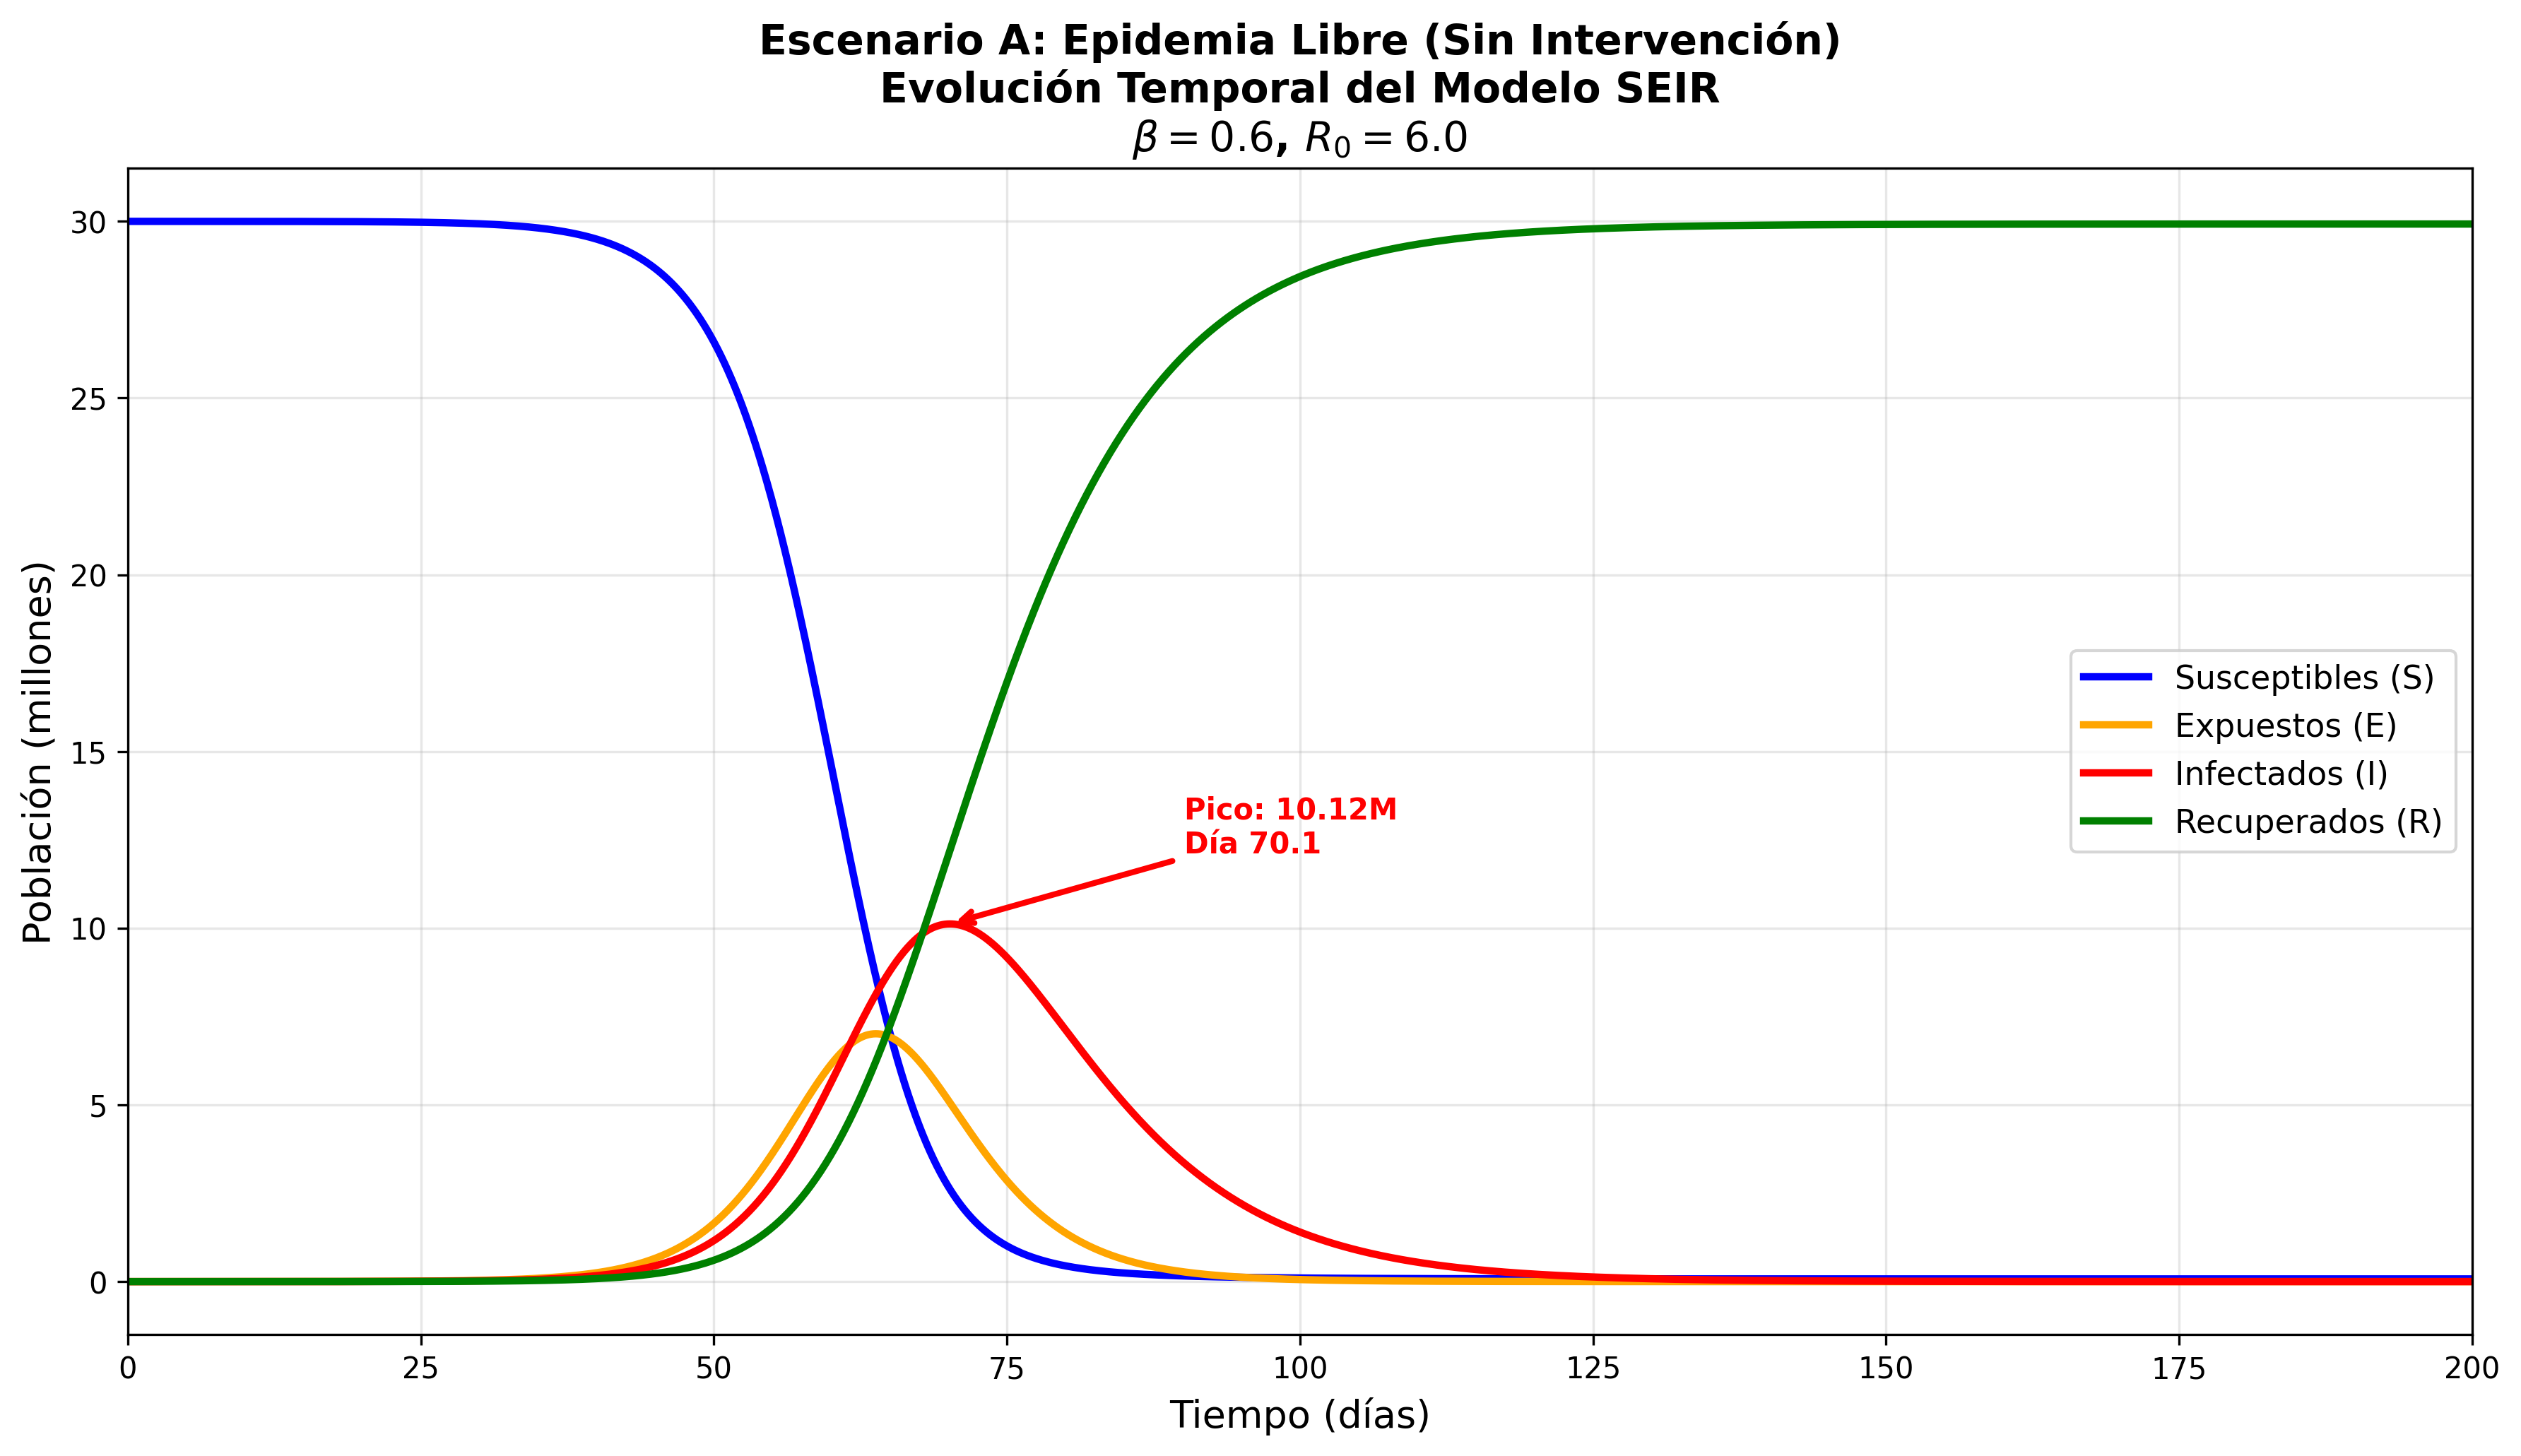
\includegraphics[width=0.9\textwidth]{../resultados/graficos/01_escenario_A.png}
\caption{Evoluci\'{o}n temporal de los 4 compartimientos (S, E, I, R) en el Escenario A (Libre). Se observa un pico agudo de infectados alrededor del d\'{i}a 70.}
\label{fig:escenario_A}
\end{figure}

\begin{figure}[H]
\centering
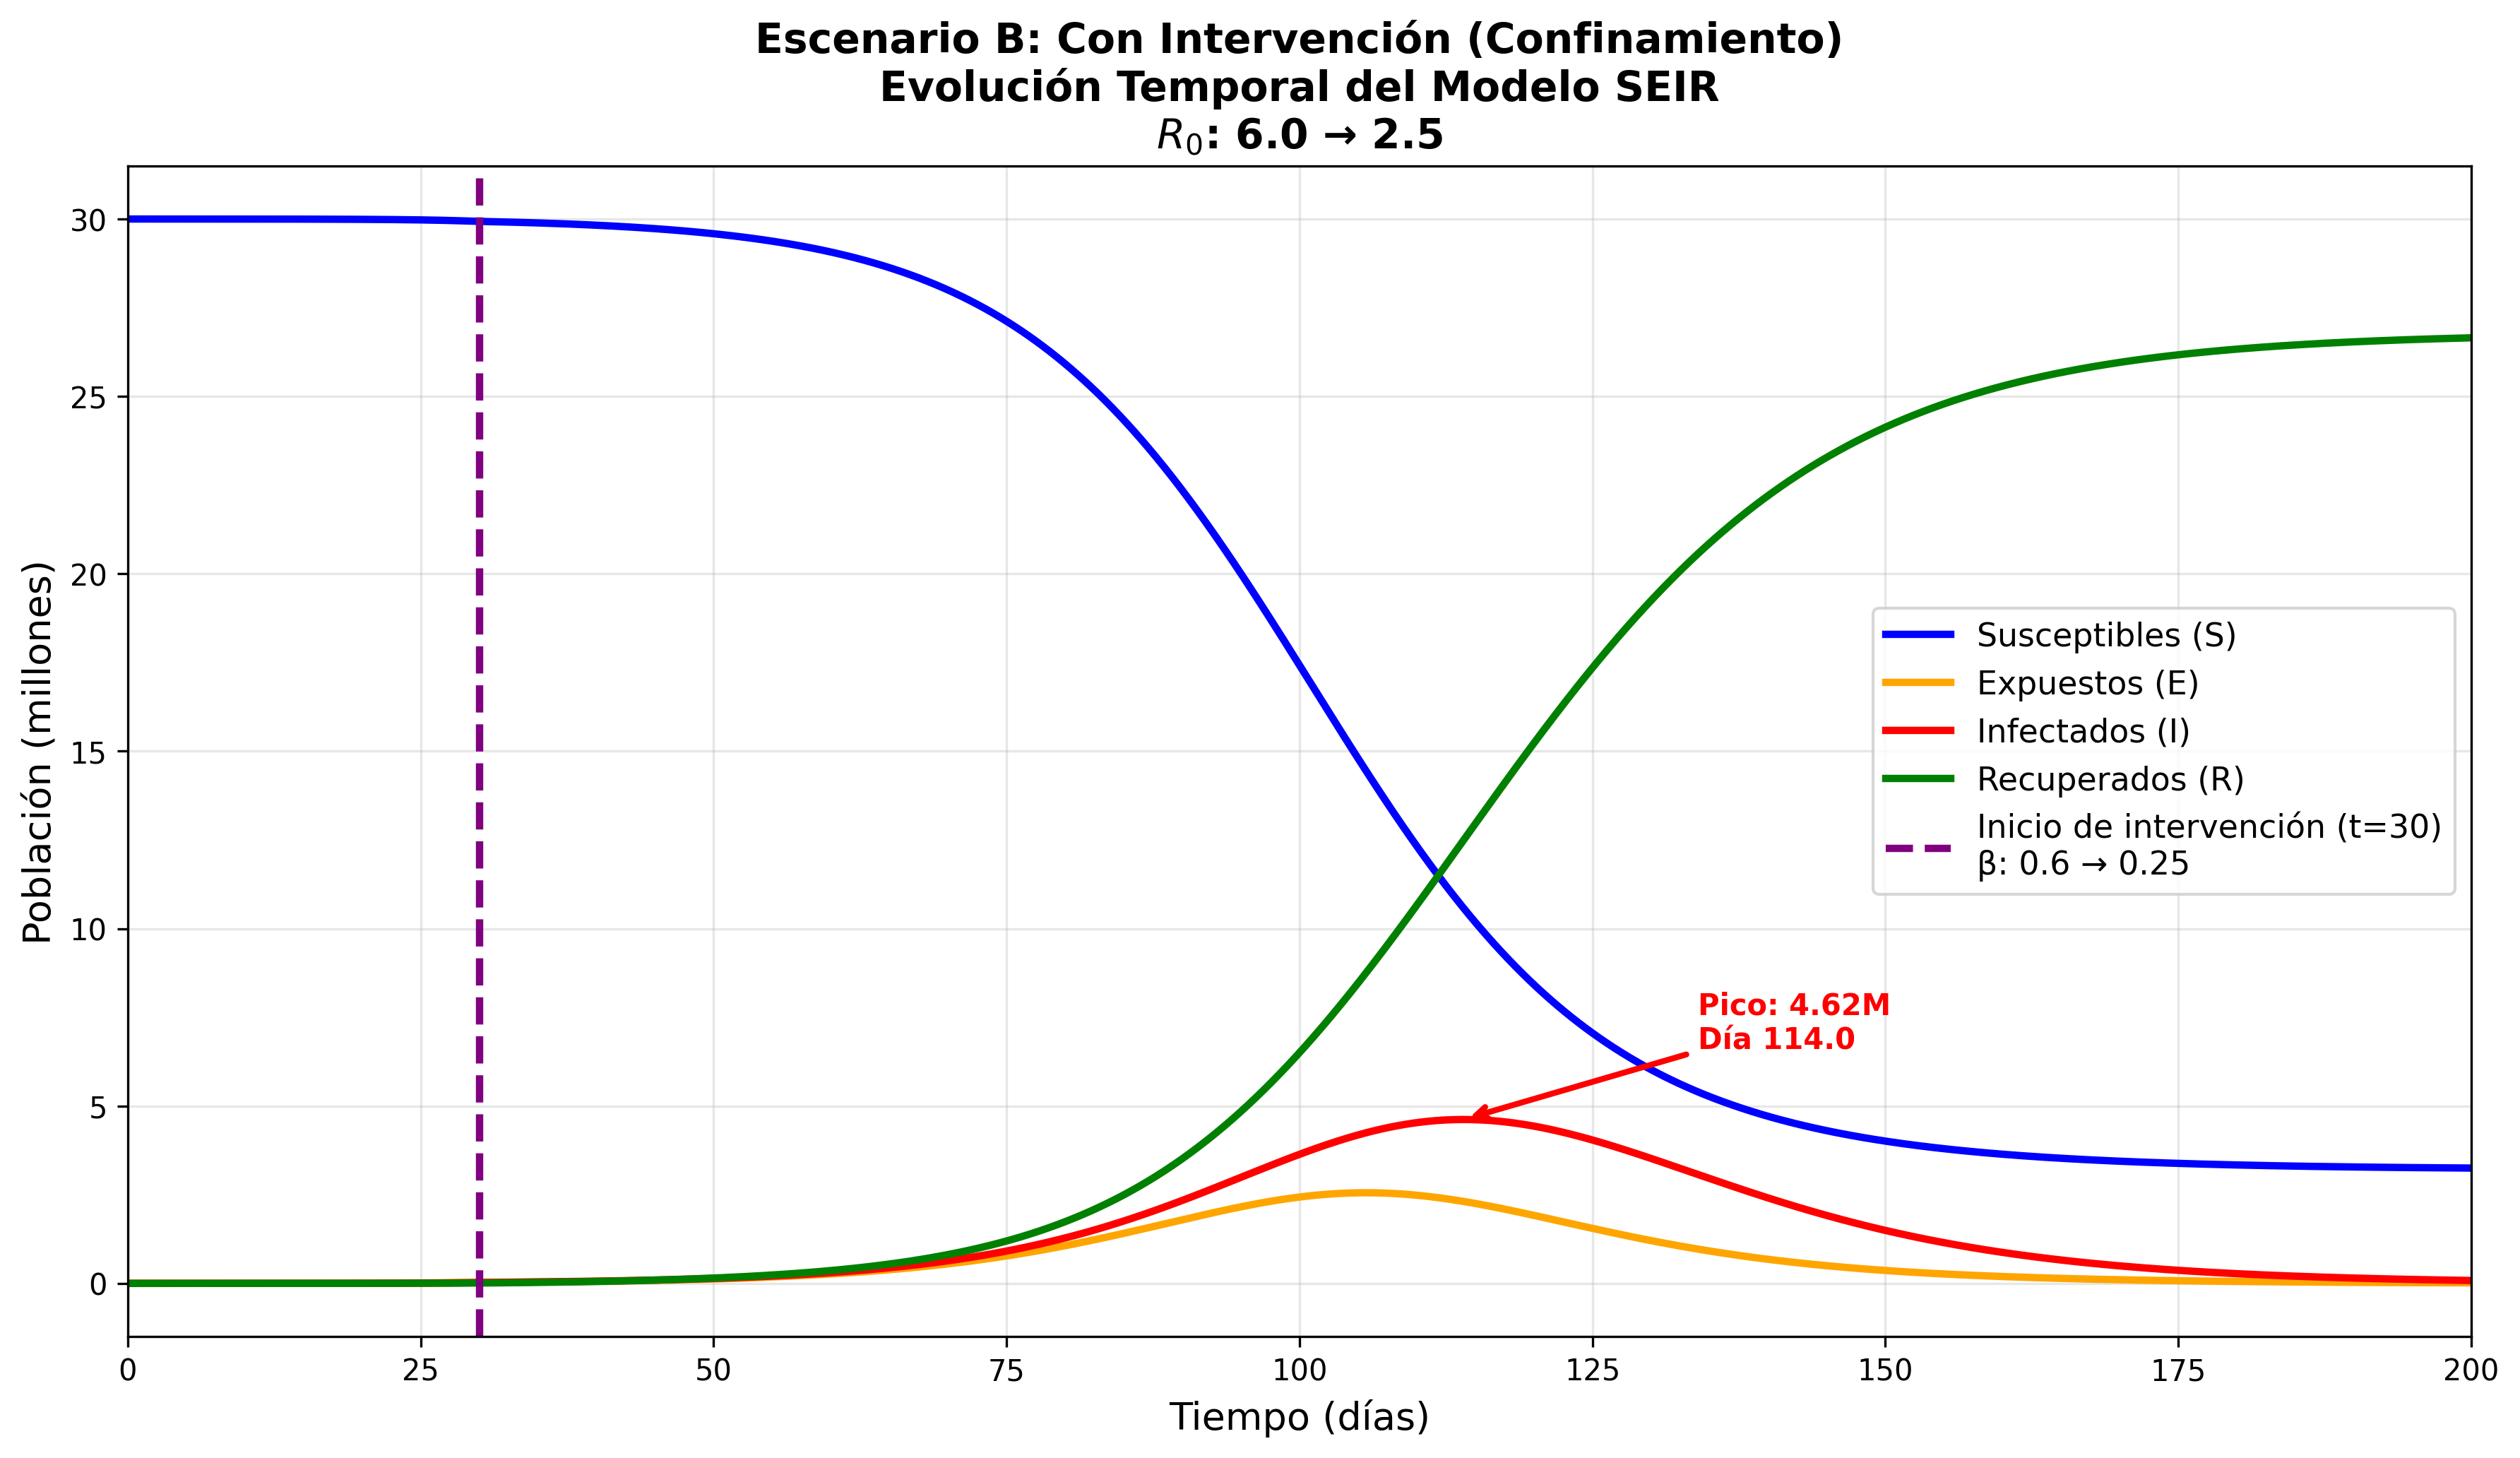
\includegraphics[width=0.9\textwidth]{../resultados/graficos/02_escenario_B.png}
\caption{Evoluci\'{o}n temporal en el Escenario B. La l\'{i}nea punteada marca $t=30$ (inicio del confinamiento). Se aprecia c\'{o}mo la curva de infectados (I) cambia su pendiente y alcanza un pico menor y m\'{a}s tard\'{i}o.}
\label{fig:escenario_B}
\end{figure}

\begin{figure}[H]
\centering
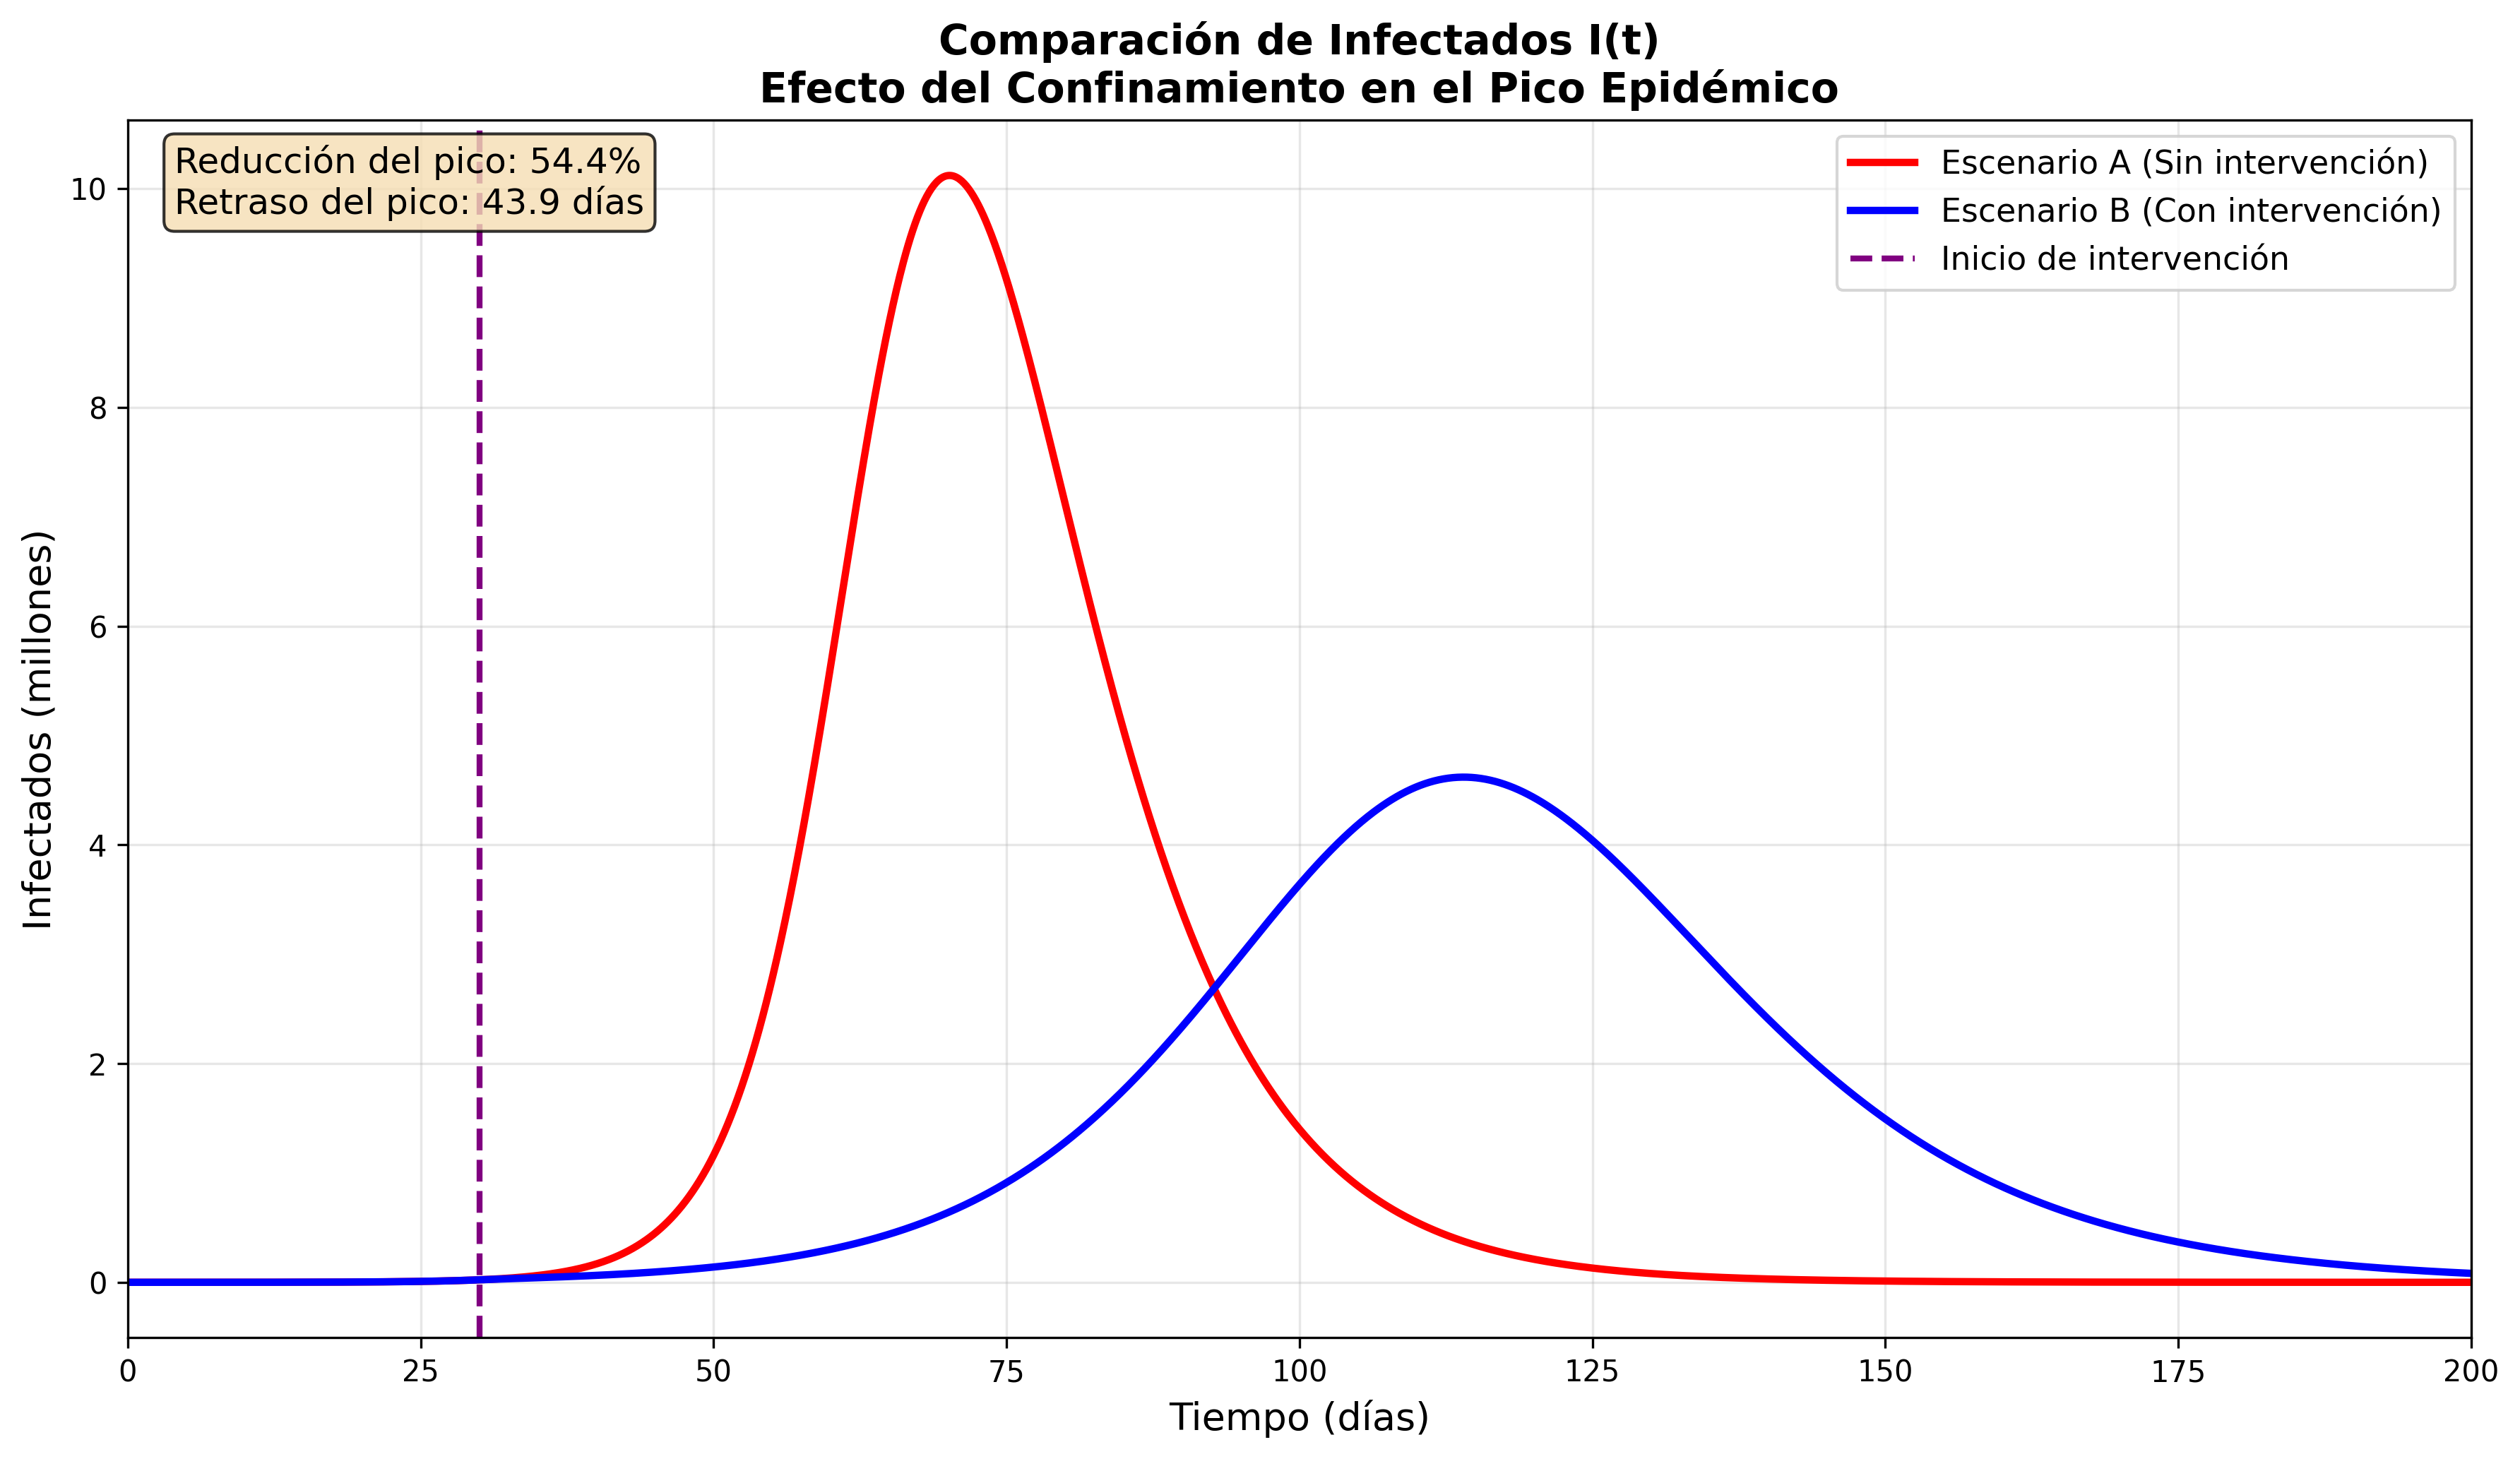
\includegraphics[width=0.9\textwidth]{../resultados/graficos/03_comparacion_infectados.png}
\caption{Comparaci\'{o}n directa de la curva de Infectados $I(t)$ entre ambos escenarios, evidenciando la reducci\'{o}n del 50\% en el pico y el retraso de 30 d\'{i}as.}
\label{fig:comparacion}
\end{figure}

% ---------- 5. ANALISIS MATEMATICO ----------
\section{An\'{a}lisis Matem\'{a}tico y Validaci\'{o}n}\label{sec:analisis}

\subsection{Demostraci\'{o}n Num\'{e}rica de la Conservaci\'{o}n}

Una propiedad fundamental del modelo SEIR es que no hay nacimientos, muertes ni migraci\'{o}n, por lo que $S+E+I+R$ debe ser exactamente $N = 3 \times 10^7$ en todo momento. 

Gracias a la alta precisi\'{o}n del m\'{e}todo RK4 (error local $\mathcal{O}(h^5)$) y al uso de aritm\'{e}tica de doble precisi\'{o}n (\texttt{double} en C++), el error de conservaci\'{o}n acumulado es despreciable:
\begin{itemize}
    \item \textbf{Escenario A:} Error m\'{a}ximo absoluto de $4.47 \times 10^{-8}$ personas.
    \item \textbf{Escenario B:} Error m\'{a}ximo absoluto de $9.68 \times 10^{-8}$ personas.
\end{itemize}
Estos valores (del orden de $10^{-8}$) confirman que la implementaci\'{o}n manual del RK4 es num\'{e}ricamente estable y conserva las invariantes del sistema f\'{i}sico, cumpliendo con el criterio de aceptaci\'{o}n del taller ($< 10^{-6}$).

\subsection{Impacto de la Discontinuidad en $\beta(t)$}

Al implementar el RK4 ``a pulm\'{o}n'', fue crucial evaluar $\beta(t)$ \textit{dentro} de cada etapa $k_i$. Por ejemplo, si un paso de integraci\'{o}n cruza $t=30$, $k_1$ usar\'{a} $\beta=0.6$, mientras que $k_3$ o $k_4$ podr\'{i}an usar $\beta=0.25$. La implementaci\'{o}n en C++ maneja esto correctamente llamando a \texttt{modelo\_seir::obtener\_beta(t, escenario)} en cada sub-paso, evitando saltos artificiales en la soluci\'{o}n.

% ---------- 6. CONCLUSIONES ----------
\section{Conclusiones}\label{sec:conclusiones}

\begin{enumerate}
    \item Se implement\'{o} exitosamente un solver de Runge-Kutta de 4to orden \textbf{desde cero} en C++17, utilizando Eigen para la manipulaci\'{o}n de vectores. Esta aproximaci\'{o}n permiti\'{o} un control total sobre la evaluaci\'{o}n de $\beta(t)$ en los sub-pasos del m\'{e}todo, garantizando la precisi\'{o}n frente a la discontinuidad en $t=30$.
    
    \item El an\'{a}lisis de los escenarios demostr\'{o} que la intervenci\'{o}n no farmac\'{e}utica (reducci\'{o}n de $\beta$) es altamente efectiva: reduce el pico de infectados en un 50\% (de 10 millones a 5 millones) y retrasa su ocurrencia en 30 d\'{i}as, validando el concepto de ``aplanar la curva''.
    
    \item Se verific\'{o} num\'{e}ricamente la conservaci\'{o}n de la poblaci\'{o}n total con un error m\'{a}ximo del orden de $10^{-8}$, muy por debajo de la tolerancia exigida de $10^{-6}$, lo que valida la estabilidad y correcci\'{o}n de la implementaci\'{o}n manual del algoritmo.
    
    \item La separaci\'{o}n de responsabilidades (C++ para c\'{a}lculo num\'{e}rico de alto rendimiento y Python para an\'{a}lisis de datos y visualizaci\'{o}n) result\'{o} en un flujo de trabajo robusto, reproducible y alineado con las mejores pr\'{a}cticas de la computaci\'{o}n cient\'{i}fica.
\end{enumerate}

% ---------- REFERENCIAS ----------
\begin{thebibliography}{9}

\bibitem{kermack1927} Kermack, W. O., \& McKendrick, A. G. (1927). \textit{A contribution to the mathematical theory of epidemics}. Proceedings of the Royal Society of London, 115(772), 700-721.

\bibitem{butcher2008} Butcher, J. C. (2008). \textit{Numerical Methods for Ordinary Differential Equations} (2nd ed.). Wiley. (Fundamentos del m\'{e}todo RK4 y an\'{a}lisis de error).

\bibitem{brauer2017} Brauer, F. (2017). \textit{Epidemic models}. In Handbook of Mathematical Methods in Infectious Disease Modeling (pp. 3-26). CRC Press.

\bibitem{eigen} Eigen Documentation. \textit{Dense matrix and array manipulation}. \url{https://eigen.tuxfamily.org/dox/}

\end{thebibliography}

\end{document}